\chapter{Fundamentals}
\label{cha:Chapter3_Fundamentals}

Length: eher 10 pages, kann auch weniger sein

Effort: ~3-4 weeks

Hier auch mehr zu Data Mining --> fundamental
Allgemeine Techniken eher knapp, je spezifischer desto detaillierter in meine Richtung
Nur Themen, die nicht originaer von mir kommen
Muss nicht jedem erklaerbar sein --> Basislevel voraussetzen
Viele Referenzen bringen, Zitate

Questions:
\begin{itemize}
\item TODO
\end{itemize}

Content
\begin{itemize}
\item Data Mining
\item Sentiment Analysis
\begin{itemize}
\item Definition/Overview
\item Approaches
\begin{itemize}
\item Lexicon-Based
\item Machine Learning \begin{itemize}
    \item Unigram vs. n-gram/bi-gram
    \item Stop words?
    \item 
\end{itemize}
\item Hybrid
\end{itemize}
\end{itemize}
\item Twitter
\begin{itemize}
\item Overview, gehoert auch dazu, etwas knapper
\item Challenges
\end{itemize}
\end{itemize}
\TODO{deutlich detaillierter}
\section{Twitter}
Twitter is a microblogging service, which allows users to send messages, so-called "tweets", containing text, media, or links. It is one of the largest social media platforms, with 330 Million monthly users in the first quartal of 2019 who post 500 million daily messages \cite{twitter:users}. It was launched in 2006 and differentiates itself from other platforms by restricting the length of a tweet. The length of a tweet was originally restricted to 140 characters until the company expanded the size to 280 characters in 2017 \cite{twitter:characters}. Due to this, Twitter offers a large number of short messages on varying topics made by varying user groups. 

Figure \ref{fig:example_tweet} shows an example of a tweet, in this case, a tweet by NASA for the Phoenix mission. An account is identified by its unique username, in the example tweet @MarsPhoenix. There are several ways to interact with a tweet. First, a tweet can be responded to. Next, a tweet can be retweeted, which shares the tweet to a user's profile, or quoted, which adds a comment to the retweet. Finally, a tweet can be liked.

\begin{figure}
    \centering
    
\includegraphics[scale=0.3]{Images/twitter_image.png}
    \caption{Picture of a tweet made by the @MarsPhoenix account. \TODO{english}}
    \label{fig:example_tweet}
\end{figure}

Due to the characteristics mentioned above of Twitter, several \TODO{TODO} can be identified.
First, the short length can be examined. Bermingham and Smeaton compared the classification of sentiment on microblogs with longer documents and concluded that it is easier to classify microblogs \cite{microblogs}.

Furthermore, informal usage of English and length restrictions frequently lead to abbreviations, slang, and misspellings, which must be considered during \TODO{feature selection}. This leads to data sparsity, as many terms appear infrequently over an entire corpus. Saif et al. observed that "93\% of the words in the tweet data occur less than 10 times" \cite[p.~3]{data_sparsity}, compared to 78\% in movie review data.


\section{Data Mining}
\TODO{text mining}
Because of the massive amounts of data that are collected every day, processing and extracting information becomes more valuable and challenging. Tan et al. describe Data Mining as "[blending] traditional data analysis methods with sophisticated algorithms for processing this abundance of data"\cite[p.~21]{DBLP:books/aw/TanSKK2019}. Data Mining faces a few challenges. First, scalability is important, as the amount of data that can be collected and stored is constantly growing. Next, dimensionality has to be considered, which describes the number of attributes a data set has. If, for example, one needs to take multiple measurements of the same data point into account, each measurement becomes an attribute. Furthermore, the types of data are becoming more complex, as data from fields such as social media, DNA research, and climate are analyzed \cite{DBLP:books/aw/TanSKK2019}.

Data Mining can be separated into two different groups. Predictive tasks try to predict an attribute value, the target variable, using other attribute values. Descriptive tasks identify patterns, such as correlation, to understand relationships in data. Predictive modeling, according to Tan et al., "refers to the task of building a model for the target variable as a function of the explanatory variable" \cite[p.~29]{DBLP:books/aw/TanSKK2019}. This can be divided into classification for discrete target variables and regression for continuous target variables. 


\TODO{maybe difference opinion, sentiment, subjectivity?}
According to Pang and Lee Sentiment Analysis "deals with the computational treatment of [...] opinion, sentiment, and subjectivity in text" \cite[p.~5]{DBLP:journals/ftir/PangL07}.  Pang and Lee suggest several applications for Sentiment Analysis, such as review-related websites, in addition to existing technologies such as recommendation systems, as well as business and government intelligence \cite[p.~8]{DBLP:journals/ftir/PangL07}.

\section{Sentiment Analysis}
Liu defines sentiment analysis, also known as opinion mining, as "the field of study that analyzes people's opinions, sentiments, appraisals, attitudes, and emotions toward entities and their attributes expressed in written text" \cite[p.~1]{liu_2015}. He states that entities include "products, services, organizations, individuals, events, issues, or topics" \cite[p.~1]{liu_2015}. He further analyzes the difference between sentiment and opinion, citing the Merriam-Webster dictionary. There, "sentiment is defined as an attitude, thought, or judgment prompted by feeling, whereas opinion is defined as a view, judgment, or appraisal formed in the mind" \cite[p.~2]{liu_2015}. Through this definition, a subtle difference can be seen, where sentiment tends to be viewed more as a feeling, while an opinion is a more concrete view. While this difference exists, Sentiment Analysis and Opinion Mining are still used interchangeably to refer to the same field. Liu differentiates the term opinion as an encompassing term that includes not only sentiment, but also additional information, such as the opinion holder. A more formal definition for an opinion, which is often used, is also provided by Liu, which is seen in Equation \eqref{eq:opinion}:
\begin{equation}
    opinion = (e, a, s, h, t),
    \label{eq:opinion}
\end{equation}
\TODO{source single entity}
where $e$ denotes an entity, $a$ is an aspect of $e$ that is targeted, $s$ is the sentiment (positive, negative, neutral), $h$ describes the opinion holder, and $t$ the time when the opinion was published \cite{liu_2015}. To further illustrate the difference, the example sentence "I like the display of my iPad Pro.", published on 07.05.2022 by Max Mustermann is considered. Here, the entity $e$ is the target of the opinion, the iPad Pro, while $a$ is the specific attribute of the iPad that the sentiment is based on, in this case, the display. Finally, the sentiment $s$ is qualified as positive, the opinion holder $h$ is Max Mustermann, and the time $t$ is 07.05.2022, resulting in the quintuple (iPad Pro, Display, Positive, Max Mustermann, 07.07.2022). If an opinion does not target a specific aspect, but rather the entire entity, the aspect is defined as "GENERAL" \cite{liu_2015}. Liu identified three different levels of analysis. The document level classifies an entire document as positive or negative, while assuming that the entire document relates to a single entity, such as in a product review. The next level is the sentence level, which determines the sentiment of each sentence. The aspect level includes the entity and aspect with which an opinion is concerned \cite{liu_2015}. On Twitter, messages are restricted to a short length, thus the difference between the document and sentence level is diminished, as a tweet will often consist of only one sentence. Furthermore, a tweet often concerns only a single entity, often identified by the presence of a word or hashtag \cite{DBLP:journals/csur/GiachanouC16}. Thus, this thesis implements Sentiment Analysis on the document/sentence level, without regarding the entity.

\begin{figure}
    \centering
    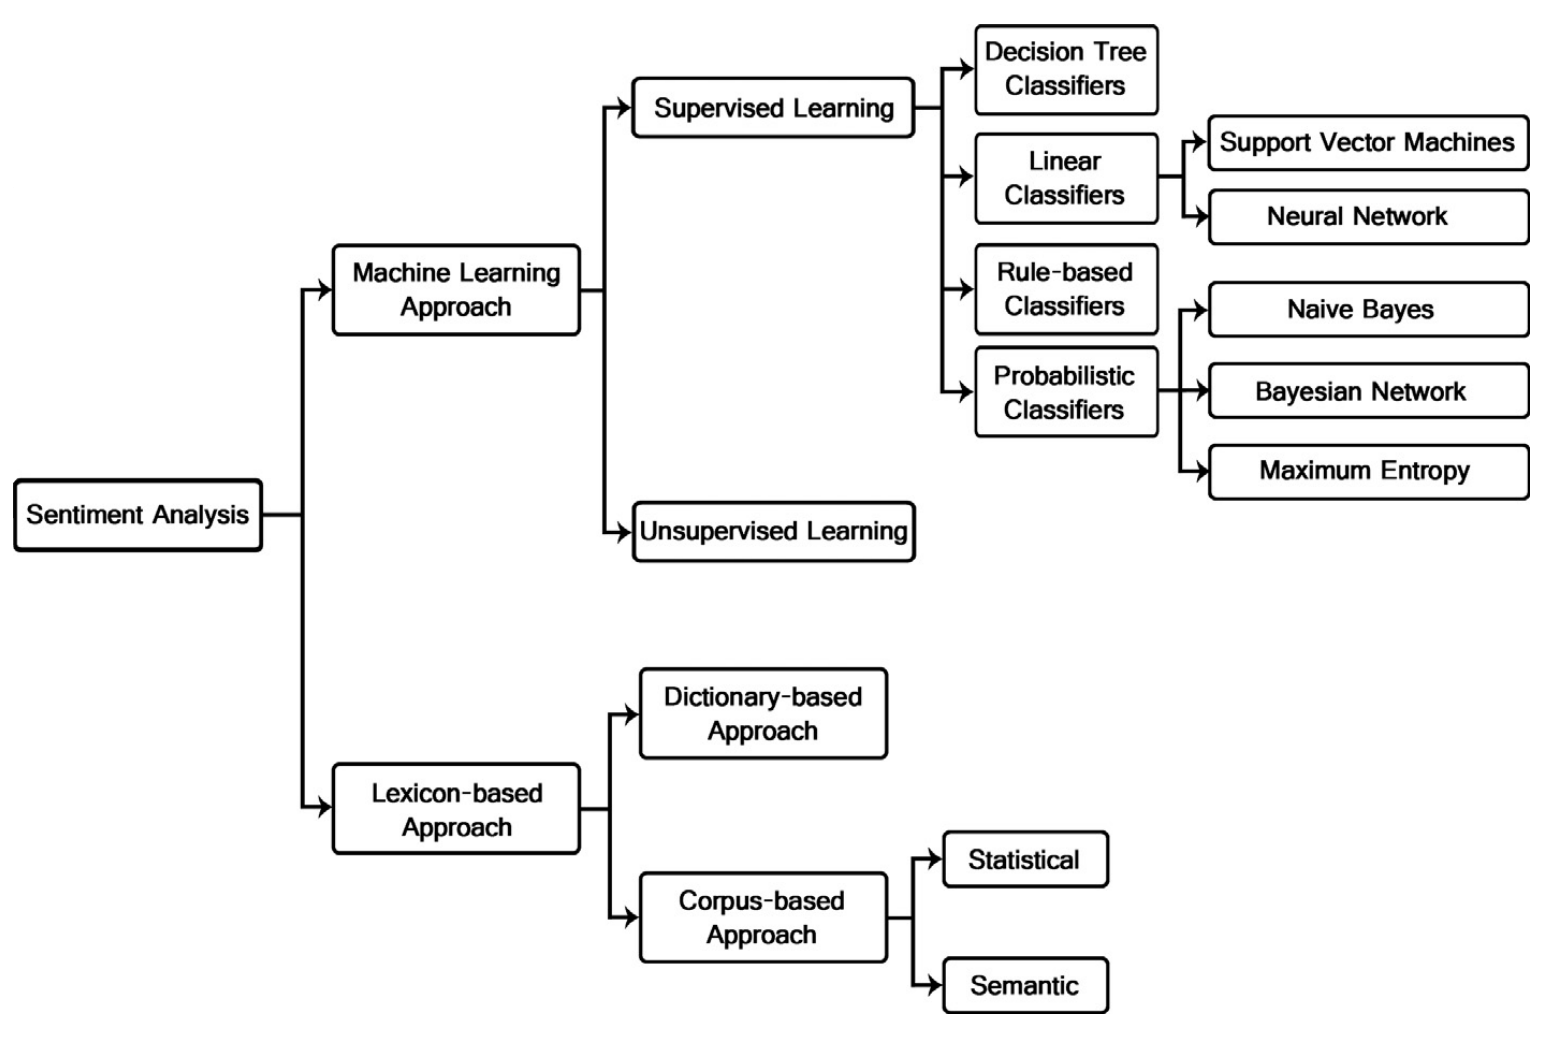
\includegraphics[scale=0.3]{Images/classification_techniques.png}
    \caption{Caption}
    \label{fig:classifiers}
\end{figure}
Medhat et al. divide classification techniques into three categories, machine learning, lexicon-based, and hybrid \cite{MEDHAT20141093}. They show the most important classifiers in Figure \ref{fig:classifiers}. Similarly, Giachanou and Crestani divide it into four categories, the above-mentioned and graph-based methods\cite{DBLP:journals/csur/GiachanouC16}. In general, the machine learning approach treats Sentiment Analysis as a text classification problem using training data to classify unknown instances. Supervised machine learning uses labeled training documents together with popular classifiers such as Naive Bayes. Because it can be difficult to generate a large number of labeled training data, unsupervised approaches are also used, which rely solely on unlabeled data \cite{MEDHAT20141093}. The lexicon-based approach makes use of a sentiment lexicon, which contains sentiment words and their values. In addition, intensifiers and negations may be used. To classify a document, all the values of sentiment words detected in the document are summed up, if the sum is positive the document is classified as negative, if the sum is 0 as neutral, and if the sum is negative as negative. By using negations and intensifiers, the sentiment values are adjusted \cite{liu_2015}.

\TODO{describe classifier types more, dictionary-based Approach vs. corpus --> dictionary building?}






